\documentclass[14pt]{extarticle}
\usepackage[french]{babel}
\usepackage{./faustin}

\usepackage{mathptmx}
\usepackage{float}
\begin{document}
\renewcommand\labelitemi{--}
\RapportUPSaclay{Rapport S105 : La maison d'édition Caribou}
\section{Introduction}
Les éditions du Caribou est une maison d'édition qui s'occupe de la production et la diffusion.
De plus la maison d'édition propose différents types d'ouvrages : romans, nouvelles ou essais.
La maison d'édition Caribou est en partenariat avec des divers auteurs et propose une large gamme littéraire.

\paragraph{Quelques chiffres}
20 employés sur 4 sites en France dont 1 à l’étranger avec le Siège social à Paris : 22 rue de Rêve, 75022 Paris.

\paragraph{Mission}
La maison a pour vocation de découvrir de nouvelles plumes, de nouveaux talents qui peuvent participer à la littérature moderne et enrichir le public avec ses œuvres. La maison du Caribou a comme but de diffuser au mieux les ouvrages des talentueux auteurs.
\subsection{Objectif du projet}
Pour développer son activité, la maison d'édition du Caribou doit créer un site internet, une plateforme de vente. La maison d'édition du Caribou a fait confiance aux étudiants de l'Université Paris-Saclay pour répondre à ce besoin et proposer un site web complet correspondant à leur métier.

Les étudiants Ecaterina GUPCA, Alice MERAUD, Jean COSTREL DE CORAINVILLE, Romain REN et Faustin MILLET se sont regroupés pour répondre à cet appel à projet. Avant de commencer le développement, nous proposons ce cahier des charges à Monsieur Ulysse et Monsieur Cyclope, co-gérants de la SARL Tabernak.

Conformément à la table des matières, ce projet décrira le fonctionnement technique de l'application, ses besoins et sa gestion des données.

\section{Analyse fonctionnelle du projet}
Voici la liste des fonctions principales et secondaires et aussi les contraintes liées à la création du site internet de la maison d'édition. Elles ont été créées et choisi en concertation avec des acteurs du milieu : libraires, clients, éditeurs et distributeurs.
\begin{figure}[h]
    \centering
    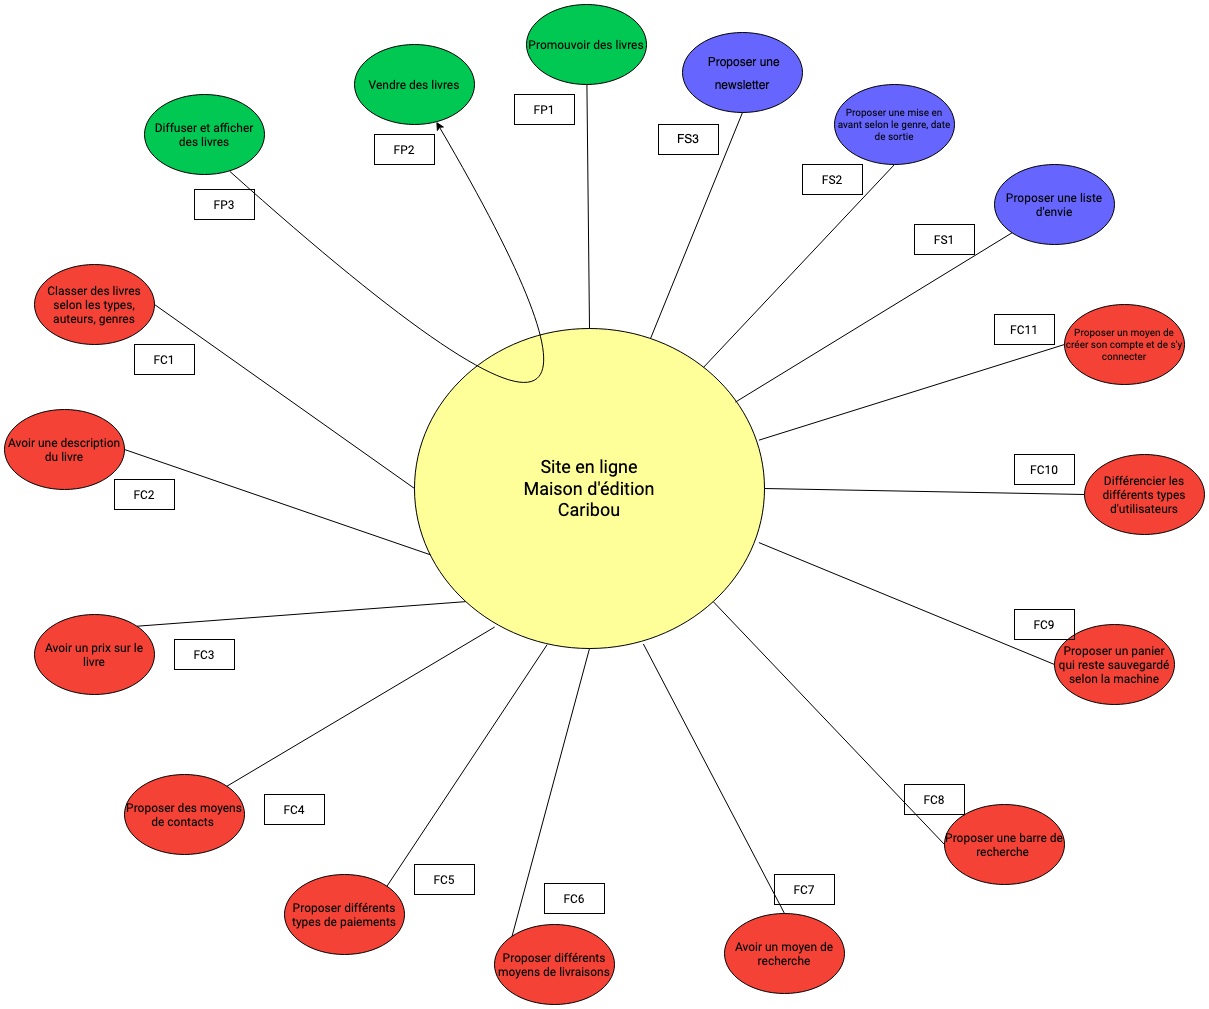
\includegraphics[width=1\linewidth]{images/diag_pieuvre.png}
    \caption{Diagramme pieuvre des interactions}
\end{figure}
\subsection{Fonctions principales}
\begin{itemize}
    \item Diffuser et proposer des livres
    \item Vendre des livres physiques et électroniques
\end{itemize}

\subsection{Contraintes}
\begin{itemize}
    \item Classer des livres selon les types, auteurs, genres
    \item Avoir une description du livre (synopsis, taille, genre, etc)
    \item Avoir un prix sur le livre
    \item Proposer différents types de paiements
    \item Proposer des moyens de contacts (email, numéro de téléphone)
    \item Proposer différents moyens de livraisons (à l'adresse, point-relais)
    \item Avoir un moyen de recherche (selon le type, auteur, genre, etc)
    \item Proposer une barre de recherche (nom du livre, auteur)
    \item Proposer un panier (achats groupés) qui reste sauvegardé selon la machine
    \item Différencier les  différents types d'utilisateurs (clients, administrateurs)
    \item Proposer un moyen de créer son compte et de s'y connecter
\end{itemize}

\subsection{Fonctions secondaires}
\begin{itemize}
    \item Proposer une newsletter
    \item Proposer une liste d'envie
    \item Proposer une mise en avant selon le genre, date de sortie
\end{itemize}

\section{Description des fonctions principales et contraintes}
Voici les différentes descriptions des fonctions principales, secondaires et contraintes décrites plus tôt.
\subsection{Fonctions principales}
\begin{itemize}
    \item \textbf{Diffuser et proposer des livres} : La fonction principale d'une maison d'édition est de publier des livres, les faire connaître pour ensuite les vendre. La maison d'édition fait la passerelle entre les auteurs des livres et les acheteurs. Fonction indispensable constituant l'essence même de la maison d'édition.
    
    \item \textbf{Vendre des livres physiques et électroniques} : Vendre des livres est la source principale de revenus d'une maison d'édition, c'est la fonction principale de la maison d'édition, elle ne peut pas vivre sans vendre des livres (que ce soit physique ou électronique).
    
    \item \textbf{Promouvoir des livres} : Indispensable pour les auteurs qui collaborent avec la maison d'édition, s'assurer de leur donner une visibilité permet de gagner une certaine confiance et d'obtenir plus de collaborateurs pour avoir davantage de livres à diffuser.
\end{itemize}

\subsection{Contraintes}
\begin{itemize}
    \item \textbf{Classer des livres selon les types, auteurs, genres} : Permettre les recherches les plus fluides et efficaces possibles est indispensable non seulement pour les potentiels acheteurs, mais pour la maison d'édition s'il a besoin de faire une recherche.

    \item \textbf{Avoir une description du livre (synopsis, taille, genre, etc)} : Permettre aux potentiels acheteurs d'avoir une description d'un livre est nécessaire pour donner l'envie d'acheter où même donner des infos complémentaires. Cela peut aussi leur faire découvrir des nouveaux livres.
    
    \item \textbf{Avoir un prix sur le livre} : Indispensable aux clients pour qu'ils puissent savoir combien ils vont dépenser pour leur achat.
    
    \item \textbf{Proposer différents types de paiements} : Il est très contraignant pour un client d'avoir un type de paiement imposé et peut même les dissuader de leur achat (ou les forcer à acheter ailleurs) et donc permettre aux clients de l'acheter quelque soit son type de paiement est nécessaire.
    
    \item \textbf{Proposer des moyens de contacts (email, numéro de téléphone)} : Pouvoir contacter la maison est primordial que ce soit pour les clients / acheteurs ou autres particuliers s'il y a un quelque besoin (service après-vente, besoin urgent).
    
    \item \textbf{Proposer différents moyens de livraisons (à l'adresse, point-relais)} : Pouvoir permettre aux clients de choisir leur moyen de livraisons est primordial, ne pas pouvoir livrer à l'adresse ou à un point-relais proche peut dissuader d'un potentiel achat (ou les forcer à acheter ailleurs).
    
    \item \textbf{Avoir un moyen de recherche (selon le type, auteur, genre, etc)} : Avoir un moyen de recherche comme un système de filtre (ou une barre de recherche) où on peut chercher selon certains critères est nécessaire non seulement pour les clients, mais aussi les administrateurs de la maison.
    
    \item \textbf{Proposer une barre de recherche (nom du livre, auteur)} : Pouvoir permettre aux utilisateurs du site de pouvoir directement chercher ce qu'ils veulent en utilisant une barre de recherche est primordial, la recherche se fera selon les titres, auteurs et aussi tags attribués aux différents livres.
    
    \item \textbf{Proposer un panier (achats groupés) qui reste sauvegardé selon la machine} : Pouvoir permettre aux clients de pouvoir avoir un panier pour acheter plusieurs produits en même temps et pouvoir le sauvegarder est primordial, ne pas en avoir un panier peut dissuader les potentiels acheteurs.
    
    \item \textbf{Différencier les différents types d'utilisateurs (clients, administrateurs)} : Contrainte importante surtout pour les administrateurs / gérants du site qui travaillent dessus pour pouvoir faire des modifications, changements sans affecter l'expérience client.
    
    \item \textbf{Proposer un moyen de créer son compte et de s'y connecter} : Permet aux utilisateurs de sauvegarder un profil qui va pouvoir garder ses préférences, panier, historique d'achat. Cette contrainte permet aux utilisateurs d'avoir une interface qui leur est dédié.
\end{itemize}

\subsection{Fonctions secondaires}
\begin{itemize}
    \item \textbf{Proposer une newsletter} : Non indispensable, mais permet une fidélisation de sa clientèle et les tiens informer des dernières sortis qui pourraient les intéresser (et potentiellement leur faire acheter).
    
    \item \textbf{Proposer une liste d'envie} : Permet aux utilisateurs de pouvoir avoir une liste à partager à leurs proches avec les différents livres qu'ils veulent avoir, c'est un panier déguisé.
    
    \item \textbf{Proposer une mise en avant selon le genre, date de sortie} : Proposer une mise en avant selon des critères  permet aux utilisateurs de découvrir directement sur la page d'accueil des œuvres et les inciter à s'intéresser et à acheter les livres mis en avant.
\end{itemize}

\section{Organigramme technique produit du site des éditions Caribou}
\begin{figure}[H]
    \centering
    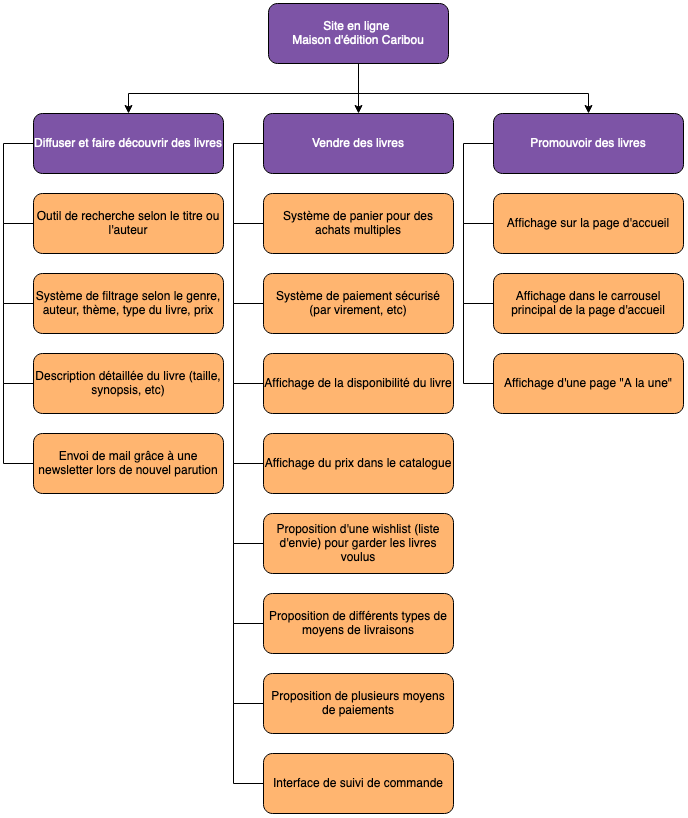
\includegraphics[width=0.8\linewidth]{images/diag_technique.png}
    \caption{Organigramme technique}
\end{figure}
\section{Modélisation de la base de données}
\subsection{Modèle Conceptuel de Données}
Le modèle conceptuel de données a été créé suivant les contraintes du site explicitées par l'organigramme technique et l'analyse fonctionnelle du projet. Il contient par exemple la remise accordée à une entreprise ou l'entité Livre qui contient un extrait et l'ISBN.
\begin{figure}[H]
    \centering
    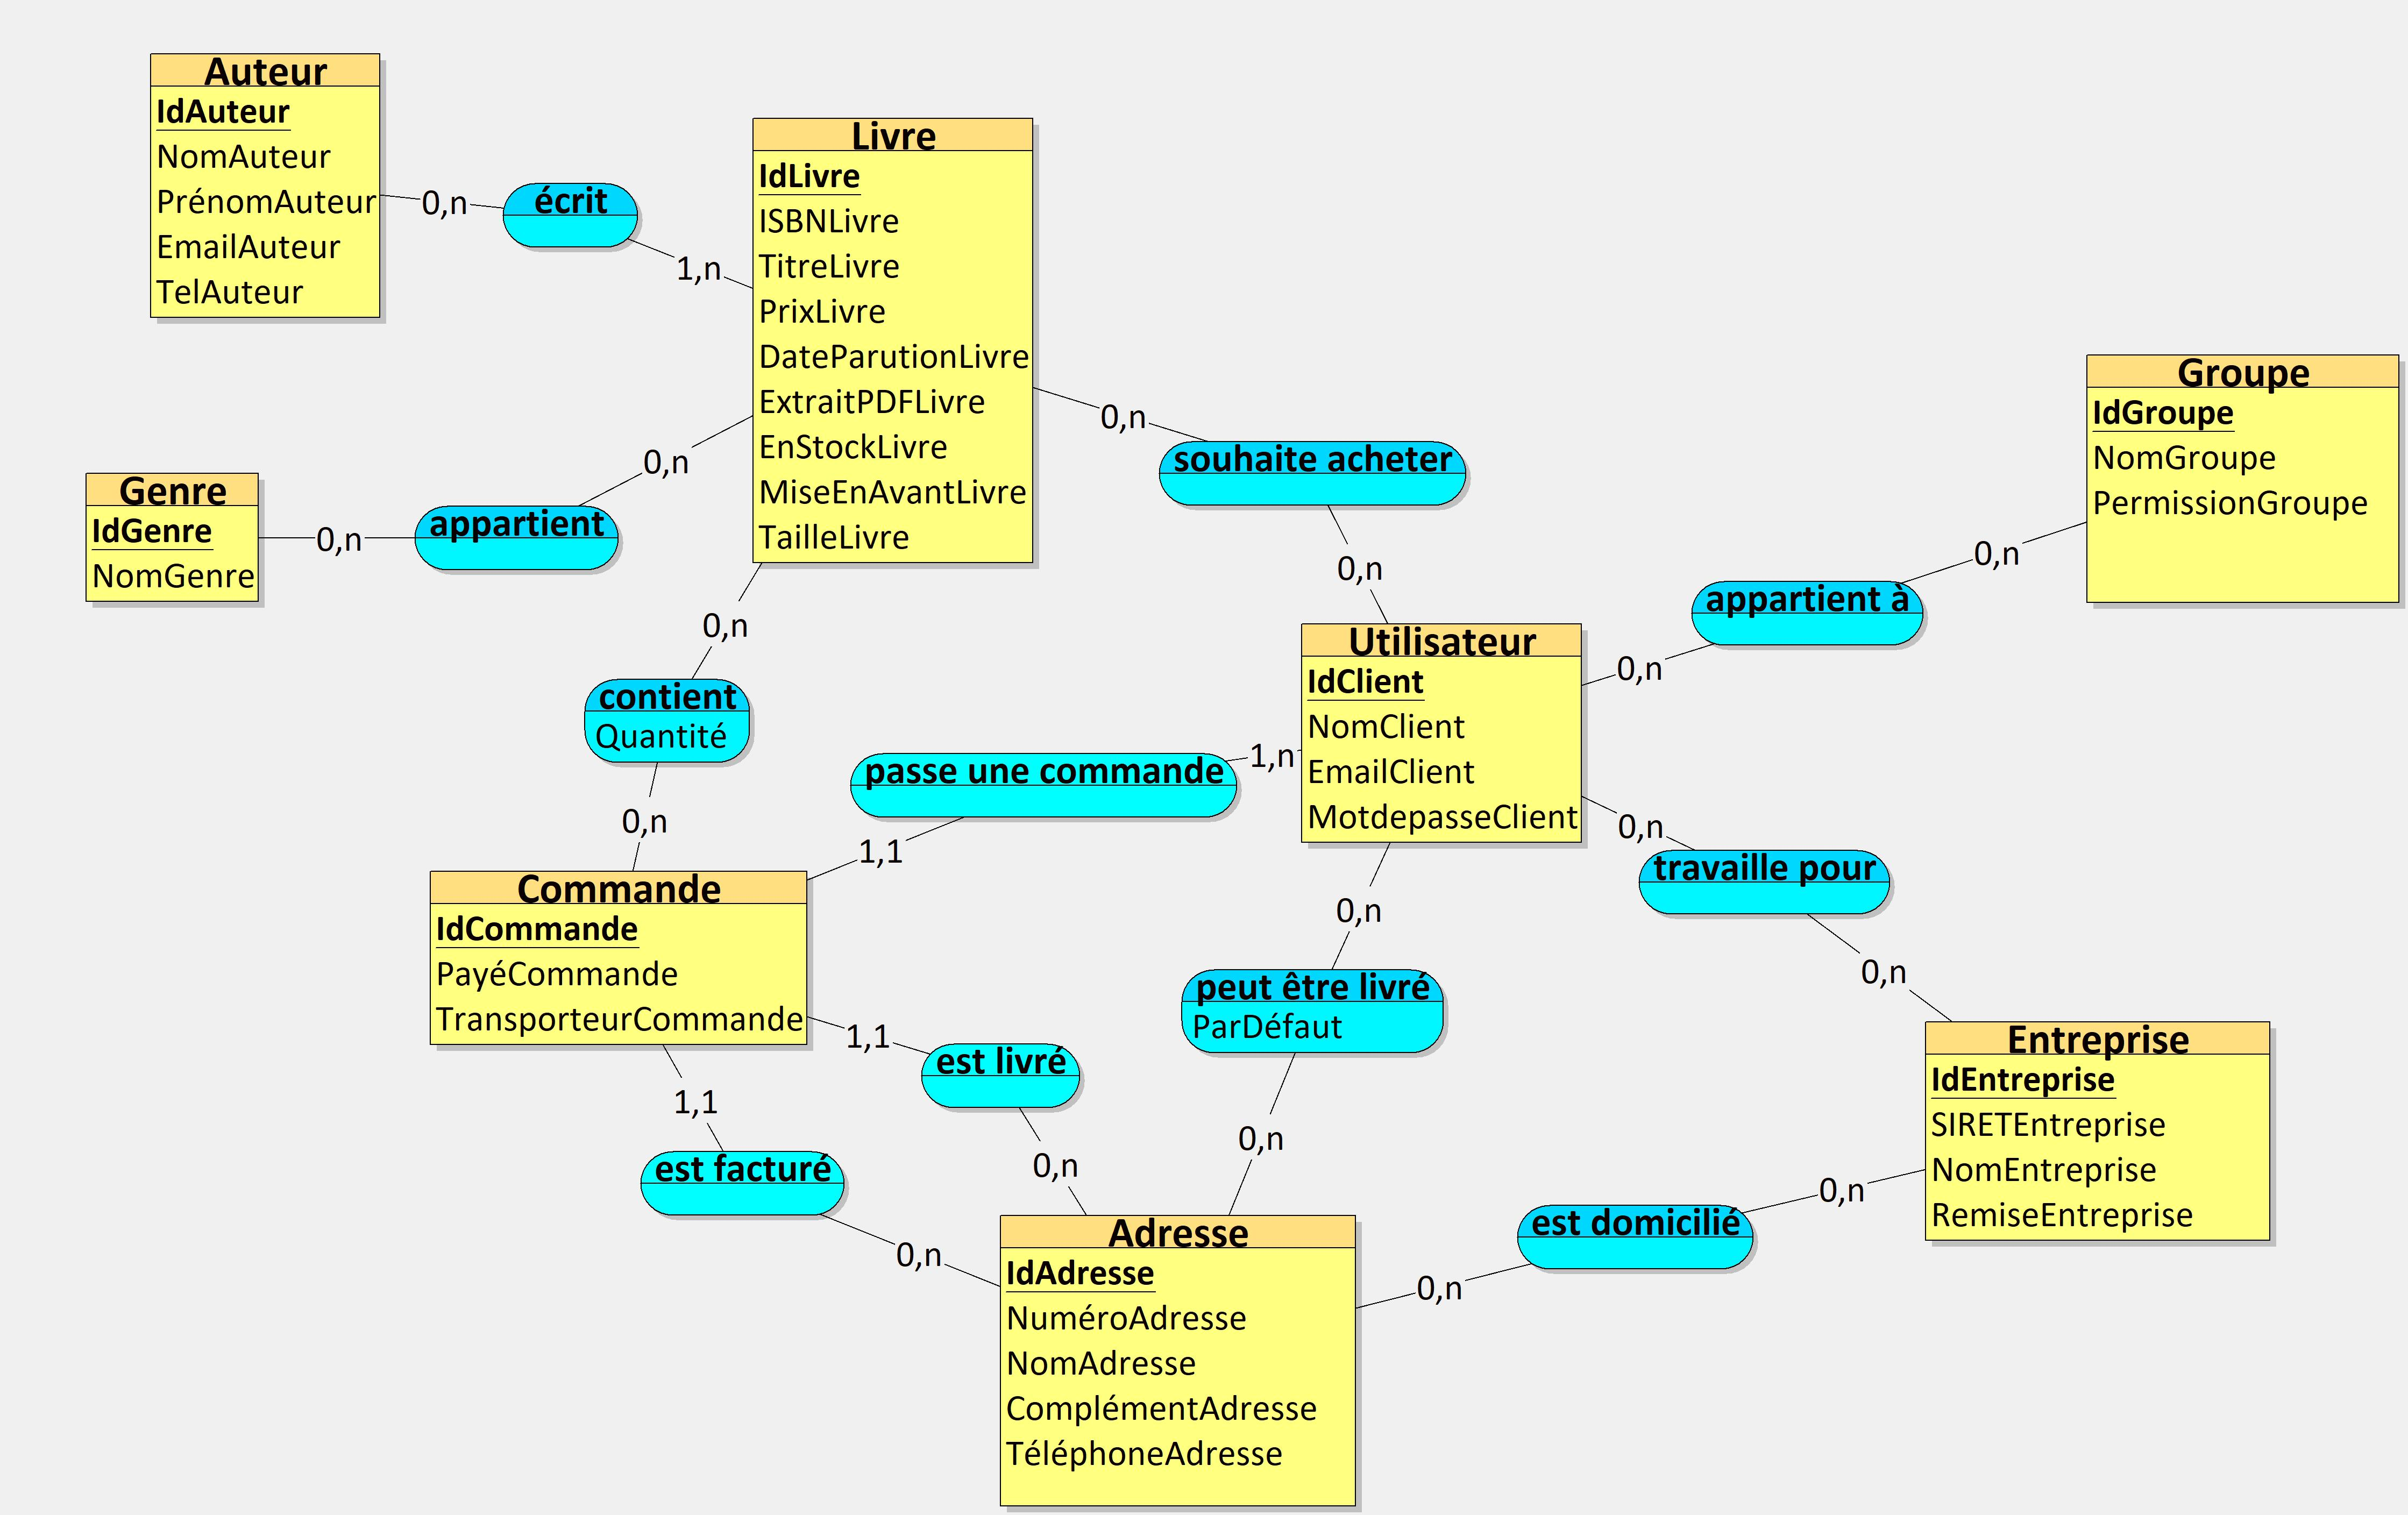
\includegraphics[width=0.9\linewidth]{images/mcd.jpg}
    \caption{Modèle Conceptuel de Données}
\end{figure}
\newpage
\subsection{Schéma relationnel}
Le schéma relationnel respecte l'ensemble des règles spécifiques au passage d'un MCD au SR.
\begin{figure}[H]
    \centering
    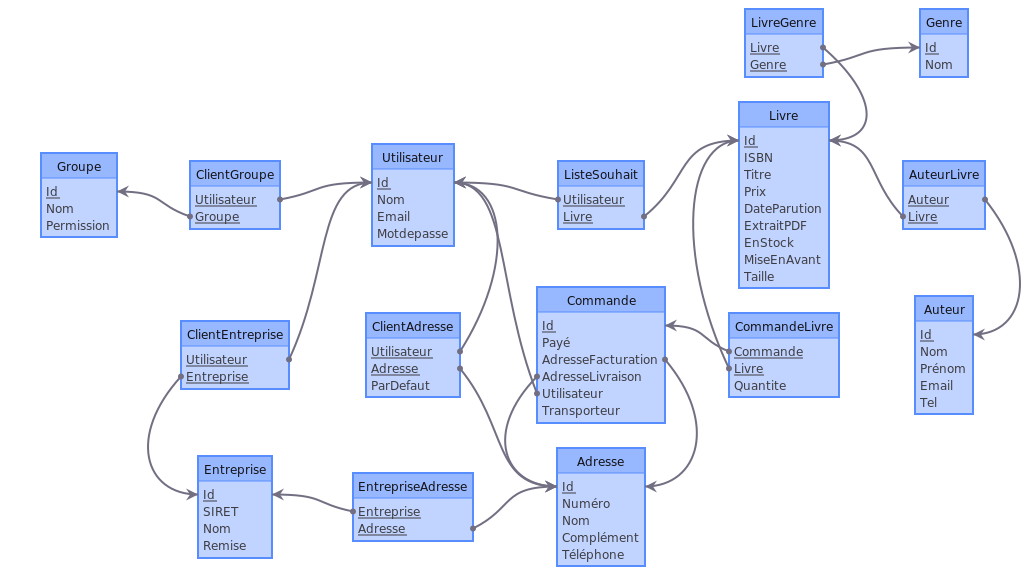
\includegraphics[width=1\linewidth]{images/sr.png}
    \caption{Schéma relationnel}
\end{figure}
\subsection{Dictionnaire de données}
Voici le dictionnaire de données lié à la base de données du site internet de la maison d'édition Caribou.
\begin{center}
    \begin{longtable}{|p{0.25\linewidth}|p{0.06\linewidth}|p{0.50\linewidth}|}
        \hline
        \textbf{Nom de la rubrique} & \textbf{Type} & \textbf{Description} \\
        \hline 
        \hline
        IdAuteur & A & Identifiant unique de l'auteur(pour éviter les homonymes) \\
        \hline
        NomAuteur & A & Nom de l'auteur \\
        \hline
        PrénomAuteur & A & Prénom de l'auteur \\
        \hline
        EmailAuteur & A & Email de l'auteur \\
        \hline
        TelAuteur & A & Numéro de téléphone de l'auteur \\
        \hline
        IdLivre & A & Identifiant unique du livre \\
        \hline
        ISBNLivre & A & ISBN du livre (Identifiant unique et international du livre) \\
        \hline
        TitreLivre & A & Titre du livre \\
        \hline
        PrixLivre & A & prix du livre \\
        \hline
        DateParutionLivre & A & Date de la parution du livre \\
        \hline
        ExtraitPDFLivre & A & Extrait PDF du livre (lien de téléchargement de l'extrait) \\
        \hline
        EnStockLivre & A &  Booléen qui permet de savoir si le livre est en stock \\
        \hline
        MiseEnAvantLivre & A & Mets en avant le livre sur la page d'accueil(Booléen 1 si le livre est sur la page d'accueil sinon 0)\\
        \hline
        TailleLivre & A & Dimension du livre(exemple "11 xH 18cm" un livre de largeur 11cm est de longueur 18cm) \\
        \hline
        IdGenre & A & Identifiant unique du genre \\
        \hline
        NomGenre & A & Nom du genre (exemple "roman policier") \\
        \hline
        IdCommande & A & Identifiant unique de la commande \\
        \hline
        PayéCommande & A &  Booléen qui indique si la commande a été payés \\
        \hline
        Transporteur
        Commande & A &  Nom de la société de transporteur qui transporte la commande (exemple "colissimo") \\
        \hline
        IdAdresse & A & Identifiant unique de l'adresse \\
        \hline
        NuméroAdresse & A & Numéro de l'adresse \\
        \hline
        NomAdresse & A & Nom de l'adresse (exemple "Rue Caribou Paris France") \\
        \hline
        ComplémentAdresse & A & Complément de l'adresse(indication d'un bis ou code du bâtiment...) \\
        \hline
        TéléphoneAdresse & A & Numéro de Téléphone du client concerné par la livraison à l'adresse \\
        \hline
        IdClient & A & Identifiant unique du client \\
        \hline
        NomClient & A & Nom du client \\
        \hline
        EmailClient & A & Email du client \\
        \hline
        MotdepasseClient & A & Mot de passe du client (exemple "MaudPassePas") \\
        \hline 
        IdGroupe & A & Identifiant unique du Groupe \\
        \hline
        NomGroupe & A & Nom du Groupe \\
        \hline
        PermissionGroupe & A & Tableau de booléen pour savoir les permissions du Groupe \\
        \hline
        IdEntreprise & A & Identifiant unique de l'entreprise \\
        \hline
        SIRETEntreprise & A & SIRET de l'entreprise \\
        \hline
        Nomntreprise & A & Nom de l'entreprise \\
        \hline
        RemiseEntreprise & A & Remise de l'entreprise \\
        \hline
        TVA & P & Taxe Valeur Ajouté \\
        \hline
        ToTalPrixPanier & C & Le prix du panier avec la formule \code{SOMME(PrixLivre+TVA)} \\
        \hline
        \caption{Dictionnaire de données}
    \end{longtable}
\end{center}

\newpage
\section{Maquettage}
La charte graphique du site a été choisi en cohérence avec l'identité de marque de Caribou. Le logo représente le célèbre animal(le caribou) et la couleur est calme et rappel la nature. Il permet de mettre en confiance l'acheteur et le fidéliser.
\begin{figure}[H]
    \centering
    
\includegraphics[width=0.8\linewidth]{images/m_accueil.png}
    \caption{Maquette de la page d'accueil du site}
\end{figure}
\begin{figure}[H]
    \centering
    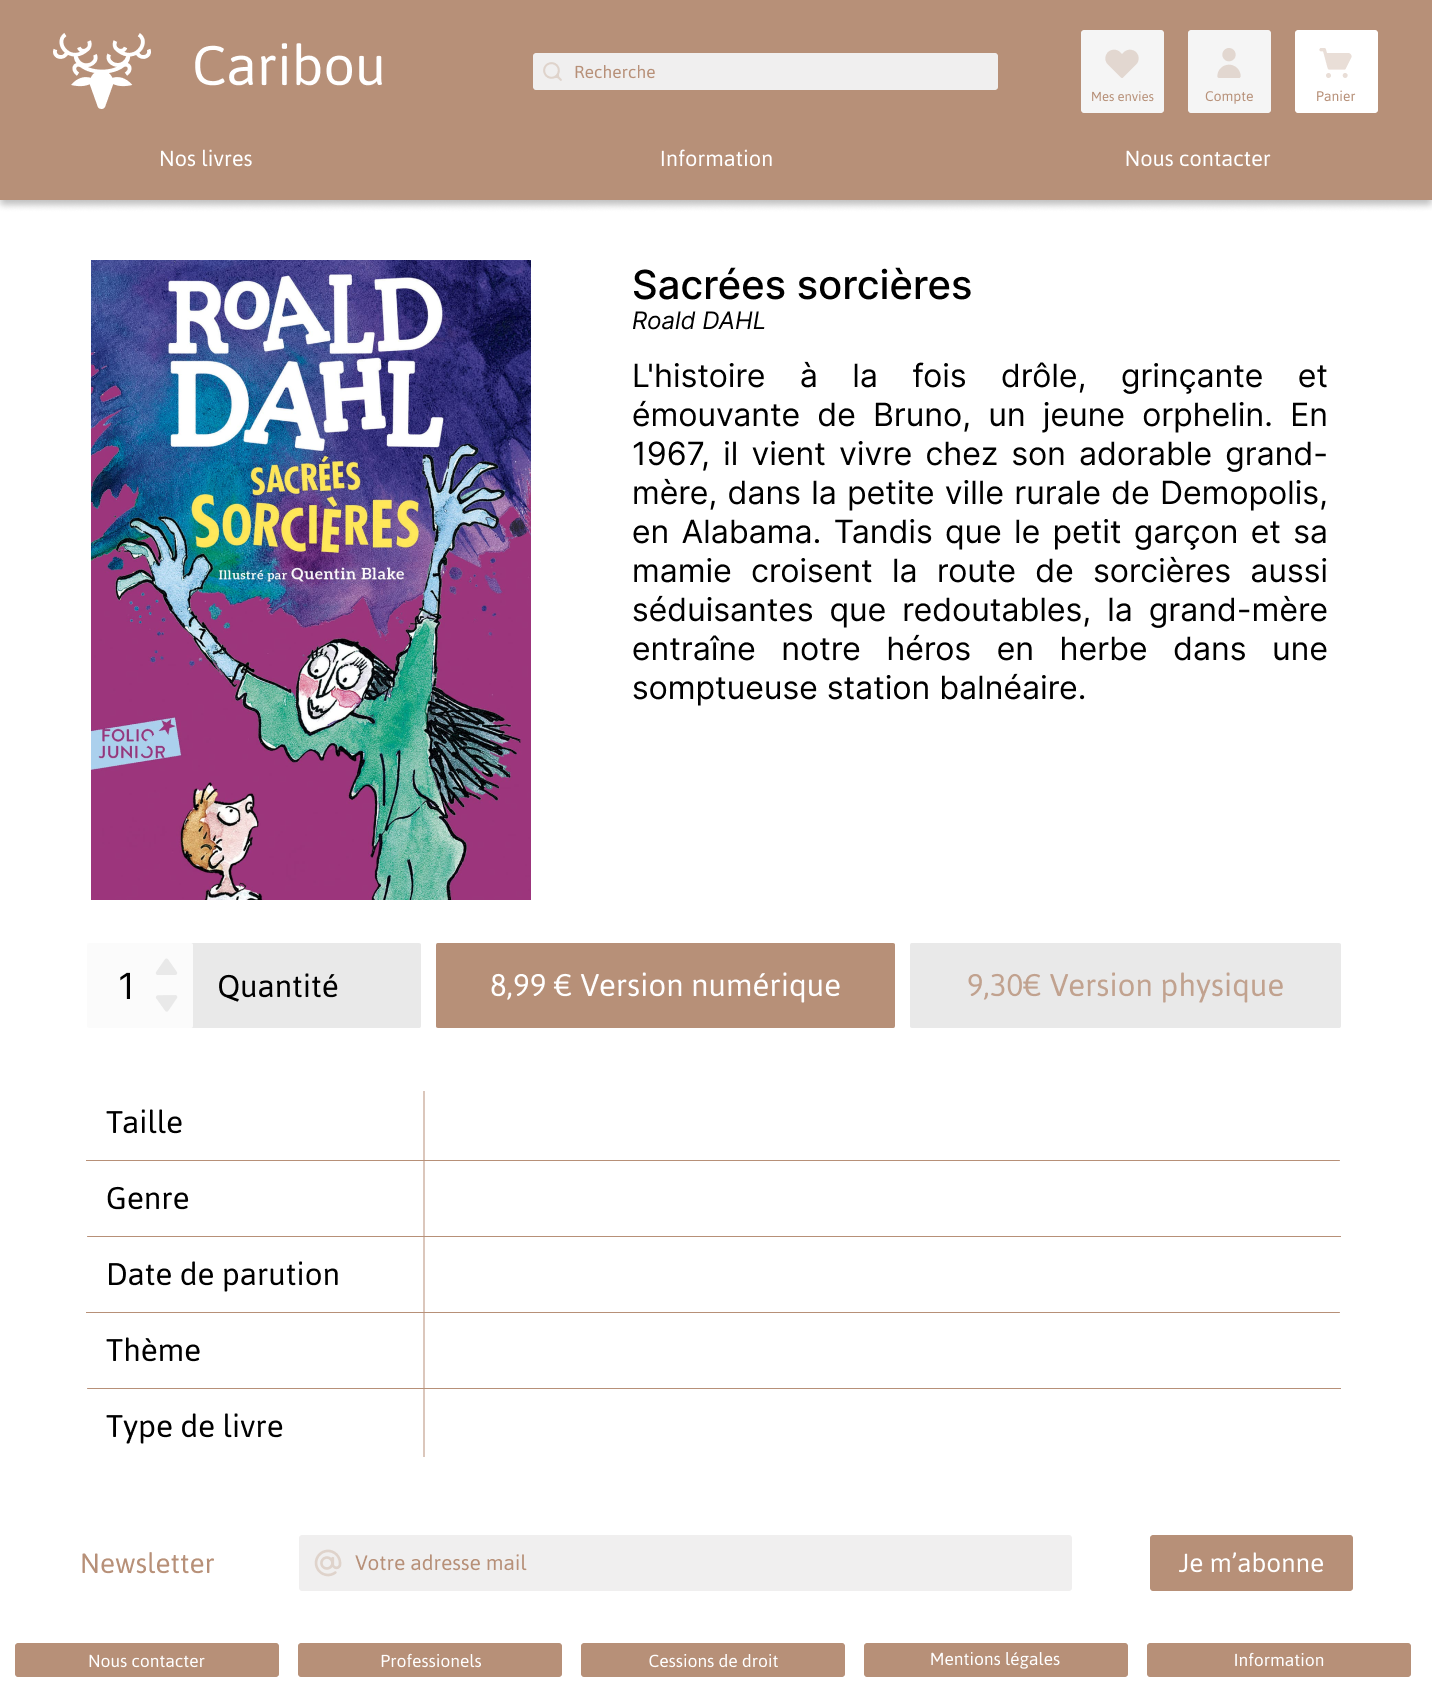
\includegraphics[width=0.8\linewidth]{images/m_livre.png}
    \caption{Maquette de la page achat d'un livre du site}
\end{figure}
\begin{figure}[H]
    \centering
    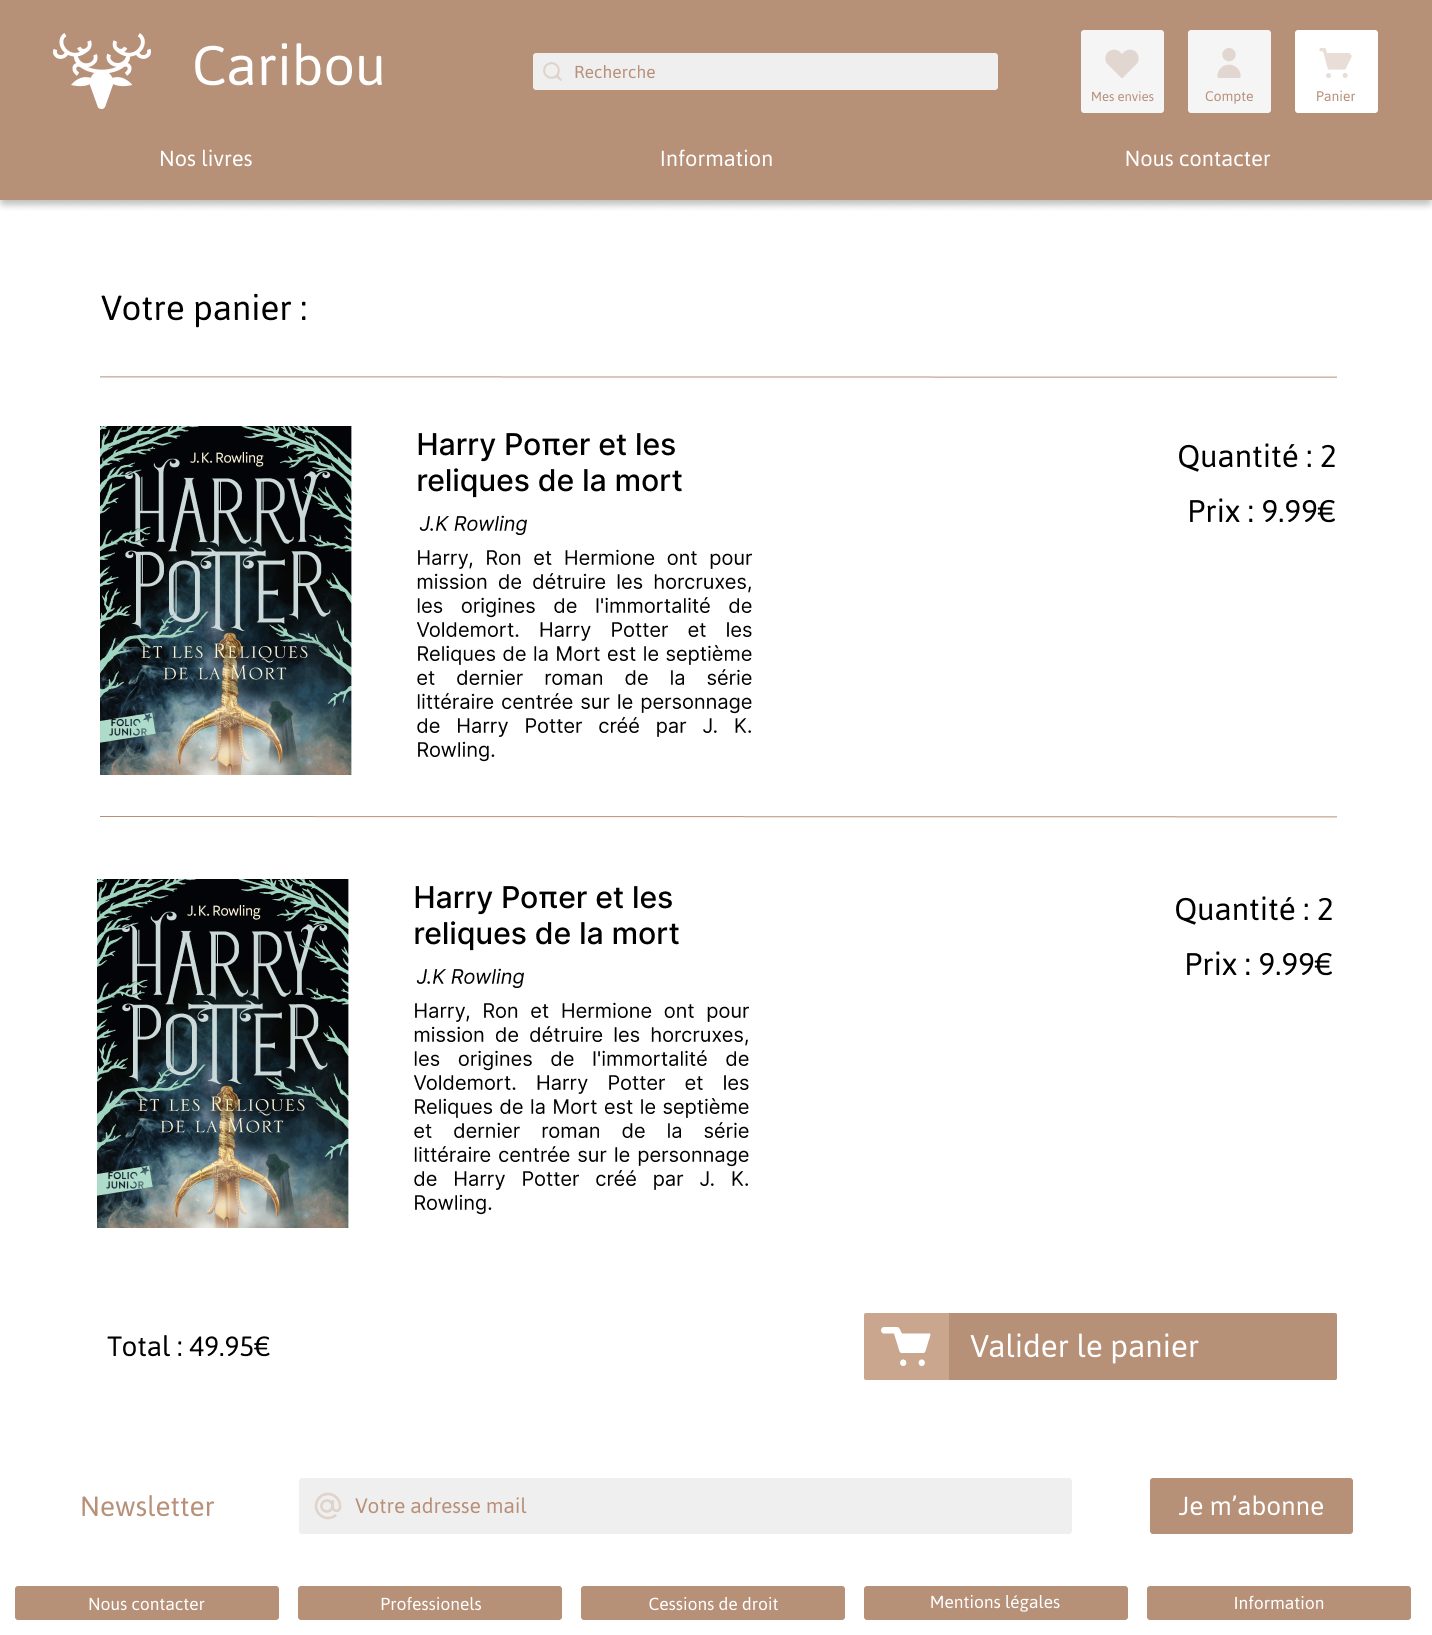
\includegraphics[width=0.8\linewidth]{images/m_panier.png}
    \caption{Maquette de la page panier du site}
\end{figure}

\newpage
\section{Processus de vente des livres}
Les acteurs du processus de vente sont les clients et le gestionnaire des stocks.
\begin{figure}[H]
    \centering
    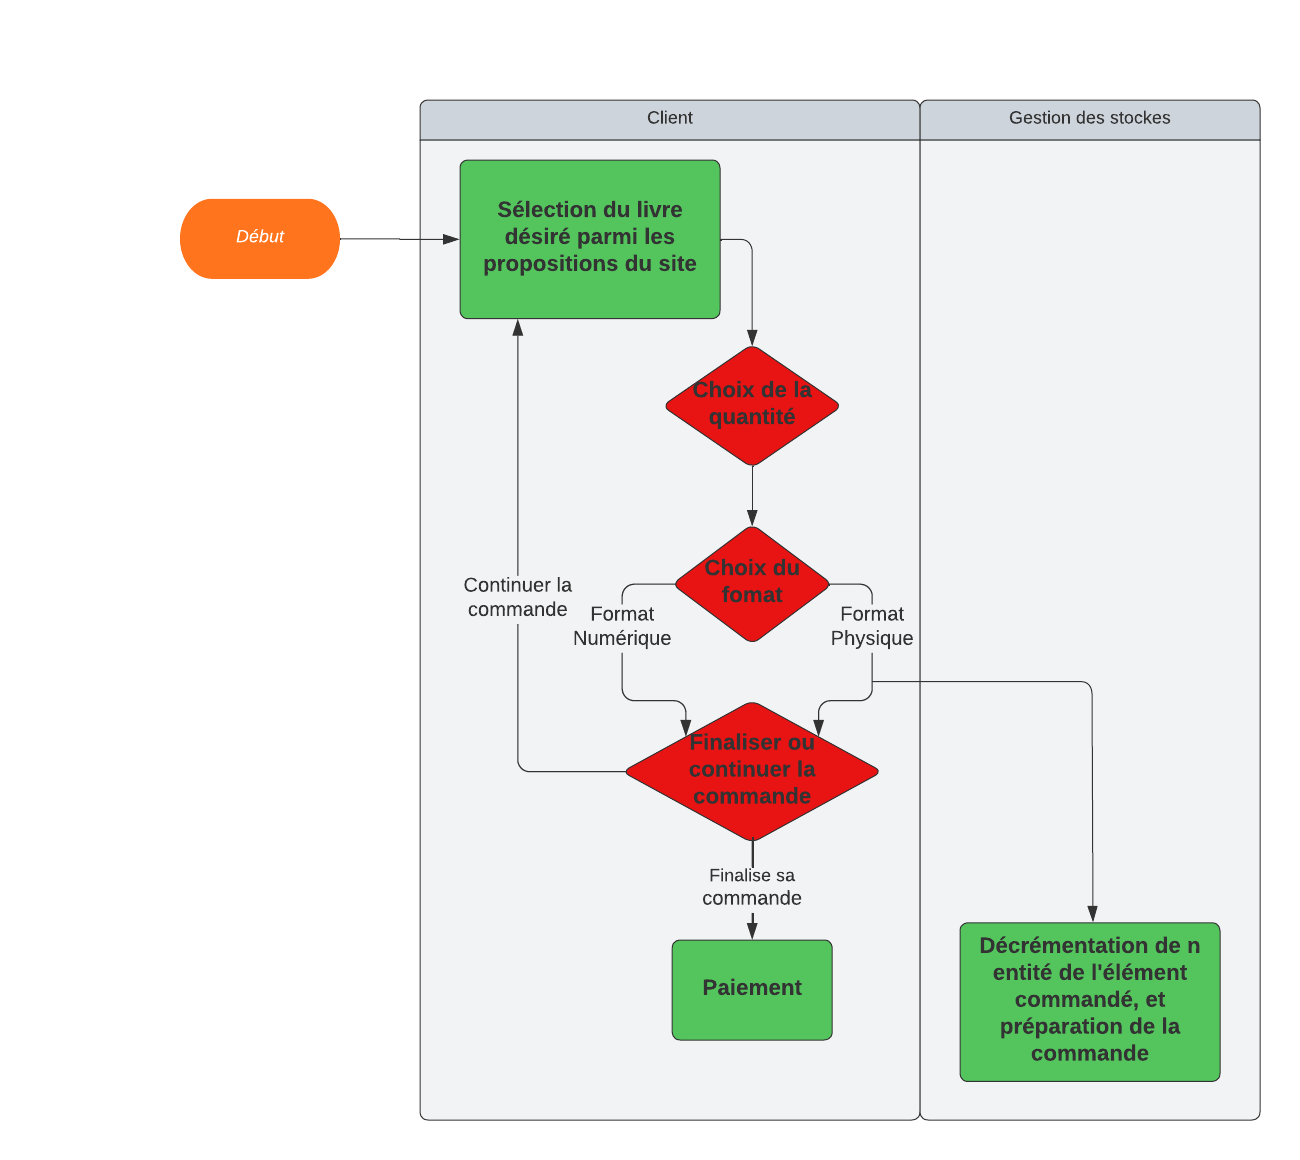
\includegraphics[width=0.8\linewidth]{images/orga.png}
    \caption{Processus de vente des livres}
\end{figure}

\subsection{Description du processus de vente}
Le client se retrouve devant un choix de livres, qu’il découvre sur le site grâce aux différentes fonctionnalités comme la recherche par nom, auteur, type, ou genre, ou bien les suggestions qui se trouvent sur la page d’accueil.

Ensuite le client a le choix entre une version numérique et une version physique, il peut choisir la quantité. Puis ajouter au panier.

Pour payer, le client doit se rendre sur son panier, mais peut aussi recommencer le processus en conservant sa commande
Et choisir son mode de paiement.

Une fois le paiement confirmé, Pour une commande physique, le stock sera décrémenté de $n$ exemplaire. Pour une commande numérique, un mail sera envoyé au client avec le document.

\section{Conclusion}
Les fondateurs de la maison d'édition pourront bénéficier du site web à partir de 28 janvier 2024. 
Ainsi l'Université Paris-Saclay présente grâce à ce cahier des charges tous les détails et besoin pour une bonne fonctionnalité du site, nous demandons Monsieur Ulysse et Cyclope de vérifier la certitude des informations et des potentielles questions/remarques.
En outre, l'Université Paris-Saclay remercie Monsieur Ulysse et Cyclope pour l'opportunité de laisser aux élèves d'examiner leur entreprise, apprendre et découvrir le milieu professionnel. Ce projet a permis d'enrichir notre culture et nous a permis d'accomplir un défi humain, passionnant et technique. Cette mise en situation a été formateur pour notre vie professionnelle future.
\end{document}